%%%%%%%%%%%%%%%%%%%%%%%%%%%%%%%%%%%%%%%%%
% University/School Laboratory Report
% LaTeX Template
% Version 3.1 (25/3/14)
%
% This template has been downloaded from:
% http://www.LaTeXTemplates.com
%
% Original author:
% Linux and Unix Users Group at Virginia Tech Wiki 
% (https://vtluug.org/wiki/Example_LaTeX_chem_lab_report)
%
% License:
% CC BY-NC-SA 3.0 (http://creativecommons.org/licenses/by-nc-sa/3.0/)
%
%%%%%%%%%%%%%%%%%%%%%%%%%%%%%%%%%%%%%%%%%

%----------------------------------------------------------------------------------------
%	PACKAGES AND DOCUMENT CONFIGURATIONS
%----------------------------------------------------------------------------------------

\documentclass{article}

\usepackage[version=3]{mhchem} % Package for chemical equation typesetting
\usepackage{siunitx} % Provides the \SI{}{} and \si{} command for typesetting SI units
\usepackage{graphicx} % Required for the inclusion of images
\usepackage{natbib} % Required to change bibliography style to APA
\usepackage{amsmath} % Required for some math elements 
\usepackage{enumerate} % Required for the enumerate function
\usepackage[americanvoltages,siunitx]{circuitikz} % Required for the drawing of circuit diagrams
\usepackage{caption}
\usepackage{graphicx}
\usepackage{subcaption}
\usepackage{xfrac}
\usepackage{float}
\usepackage{enumitem}

\setlength\parindent{0pt} % Removes all indentation from paragraphs

\renewcommand{\labelenumi}{\alph{enumi}.} % Make numbering in the enumerate environment by letter rather than number (e.g. section 6)

%\usepackage{times} % Uncomment to use the Times New Roman font

%----------------------------------------------------------------------------------------
%	DOCUMENT INFORMATION
%----------------------------------------------------------------------------------------

\title{Electrical Circuit Analysis \\ Practical 2 - Low Pass Filters \\ ENG223} % Title

\author{Shane \textsc{Reynolds}} % Author name

\date{\today} % Date for the report

\begin{document}

\maketitle % Insert the title, author and date

\begin{center}
\begin{tabular}{l r}
Date Performed: & September 8, 2015 \\ % Date the experiment was performed
Instructor: & Dr Kamal Debnath % Instructor/supervisor
\end{tabular}
\end{center}

% If you wish to include an abstract, uncomment the lines below
% \begin{abstract}
% Abstract text
% \end{abstract}

%----------------------------------------------------------------------------------------
%	SECTION 1
%----------------------------------------------------------------------------------------

\section{Objective}

To develop an understanding of low-pass filter operation through the derivation of a theoretical transfer function and theoretical cut-off frequency. Theoretical estimates will be tested through the collection of experimental evidence.

\subsection{Background}
\label{definitions}

\begin{description}
\item[Transfer function for RC low pass filter]
Figure 1 shows an RC circuit with the output voltage taken over the capacitor. This set-up is called a low-pass filter. This type of filter allows low frequency voltage signals to pass through from input to output, however, high frequency voltage signals are attenuated.

%Circuit Diagram
\begin{figure}[H]
	\centering
	\ctikzset {bipoles/length=.8cm}
	\begin{circuitikz}[scale=0.6]
		
		\draw (0,0)
		to [sV, l=$V_{in}$] (0,4)
		to [R, l=$R$] (4,4)
		to [C, v^<=$C$] (4,0)
		to [short] (0,0)
		;
		
	\end{circuitikz}
	\captionof{figure}{Series RC circuit with Sinusoidal Input Voltage}
	\label{fig:figure2}
\end{figure}

Consider the RC circuit in figure 1 with input voltage $V_{in} = V_m \cos(\omega t - \phi)$. In general, to calculate the output voltage, $V_{out}$, we exploit impedance models in the circuit's steady state. The impedance of the resistor is given by $Z_R = R$ and the impedance of the capacitor is given by $Z_C = \frac{1}{j \omega C}$, where $\omega$ is the frequency of the input voltage. Since the elements are in series, we can use the voltage divider arrangement:

\begin{align*}
	V_{out} &= \frac{Z_C}{Z_C + Z_R} V_{in} \\
	\frac{V_{out}}{V_{in}} &= \frac{Z_C}{Z_C + Z_R} \\
	& = \frac{\frac{1}{j \omega C}}{R + \frac{1}{j \omega C}} \\
	&= \frac{1}{j \omega C}\frac{j \omega C}{R j \omega C + 1} \\
	&= \frac{1}{1 + j \omega RC}
\end{align*}

This is the transfer function and is written as:

\begin{align}
	H(\omega) = \frac{1}{1 + j \omega RC}
\end{align}

This expression can be written in phasor form as follows:

\begin{align*}
	H(\omega) &= \frac{1 \angle 0 \si{\degree}}{\sqrt{1 + (\omega R C)^2} \angle \arctan (\frac{\omega RC}{1})} \\
	&= \frac{1 \angle 0 \si{\degree}}{\sqrt{1 + (\omega R C)^2} \angle \arctan (\omega RC)}
\end{align*}

Hence, the magnitude of the transfer function is given by:

\begin{align}
	|H(\omega)| = \frac{1}{\sqrt{1 + (\omega R C)^2}}
\end{align}

And the phase angle of the transfer function is given by:

\begin{align}
	\angle H(\omega) = - \arctan (\omega RC)
\end{align}

A plot of both the magnitude of the transfer function and the phase angle can be seen in figure 2.

\begin{center}
	\begin{figure}[H]
		\begin{minipage}{0.6\textwidth}
			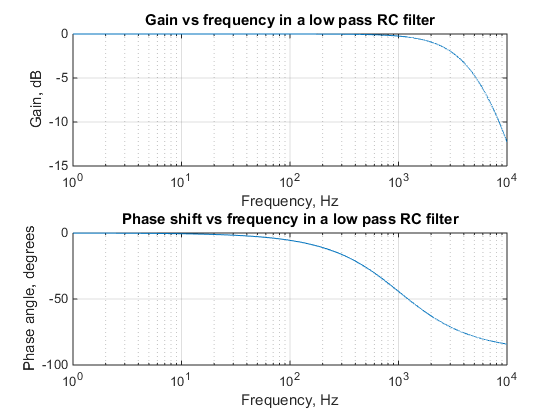
\includegraphics[scale=0.8]{bode1}
			\captionof{figure}{Theoretical bode plots for low pass RC filter}
		\end{minipage}
	\end{figure}
\end{center}

\item[Cut-off frequency for RC low pass filter]
The definition of cut-off frequency that has been widely used by electrical engineers is the frequency for which the transfer function magnitude is decreased by the factor of $\frac{1}{\sqrt{2}}$ from its maximum value. That is:

\begin{align*}
	|H(\omega_c)| = \frac{1}{\sqrt{2}}H_{max}
\end{align*}

For a low pass RC circuit, the magnitude of the transfer function is at its maximum when $\omega = 0$, that is $H_{max} = 1$. Hence, setting $|H(\omega_c)|$ equal to $\frac{1}{\sqrt{2}}$ we get:

\begin{align*}
	\frac{1}{\sqrt{1 + (\omega_c R C)^2}} &= \frac{1}{\sqrt{2}} \\
	\sqrt{1 + (\omega_c R C)^2} &= \sqrt{2} \\
	1 + (\omega_c R C)^2 &= 2 \\
	(\omega_c RC)^2 &= 2 - 1 \\
	\omega_c RC &= 1 \\
\end{align*}

Hence, for a low pass RC circuit, the cut off frequency is given by:

\begin{align}
	\omega_c = \frac{1}{RC}
\end{align}

Now, suppose the RC circuit was constructed using a 330 $\si{\ohm}$ resistor and a 0.47 $\si{\micro \farad}$ capacitor. The cut off frequency in radians per second would be:

\begin{align*}
	\omega_c &= \frac{1}{RC} \\
	&= \frac{1}{330 \times 0.47e^(-6)} \\
	&= 6447.45 \si{\sfrac{\radian}{\second}} \\
	&= 1026.14 \si{\hertz}
\end{align*}


\item[Transfer function for RL low pass filter]
Figure 2 shows an RL circuit with the output voltage taken over the resistor. This set-up is called a low-pass filter. This type of filter allows low frequency voltage signals to pass through from input to output, however, high frequency voltage signals are attenuated.

%Circuit Diagram
\begin{figure}[H]
	\centering
	\ctikzset {bipoles/length=.8cm}
	\begin{circuitikz}[scale=0.6]
		
		\draw (0,0)
		to [sV, l=$V_{in}$] (0,4)
		to [L, l=$L$] (4,4)
		to [R, v^<=$R$] (4,0)
		to [short] (0,0)
		;
		
	\end{circuitikz}
	\captionof{figure}{Series RL circuit with Sinusoidal Input Voltage}
	\label{fig:figure2}
\end{figure}

Consider the RL circuit in figure 1 with input voltage $V_{in} = V_m \cos(\omega t - \phi)$. In general, to calculate the output voltage, $V_{out}$, we exploit impedance models in the circuit's steady state. The impedance of the resistor is given by $Z_R = R$ and the impedance of the inductor is given by $Z_L = j \omega L$, where $\omega$ is the frequency of the input voltage. Since the elements are in series, we can use the voltage divider arrangement:

\begin{align*}
V_{out} &= \frac{Z_R}{Z_L + Z_R} V_{in} \\
\frac{V_{out}}{V_{in}} &= \frac{Z_R}{Z_L + Z_R} \\
& = \frac{R}{R + j \omega L} \\
\end{align*}

This is the transfer function and is written as:

\begin{align}
H(\omega) = \frac{R}{R + j \omega L}
\end{align}

This expression can be written in phasor form as follows:

\begin{align*}
H(\omega) &= \frac{R}{\sqrt{R^2 + (\omega L)^2} \angle \arctan(\frac{\omega L}{R})} \\
\end{align*}

Hence, the magnitude of the transfer function is given by:

\begin{align}
|H(\omega)| = \frac{R}{\sqrt{R^2 + (\omega L)^2}}
\end{align}

And the phase angle of the transfer function is given by:

\begin{align}
\angle H(\omega) = - \arctan (\frac{\omega L}{R})
\end{align}

A plot of both the magnitude of the transfer function and the phase angle can be seen in figure 4.

\begin{center}
	\begin{figure}[H]
		\begin{minipage}{0.6\textwidth}
			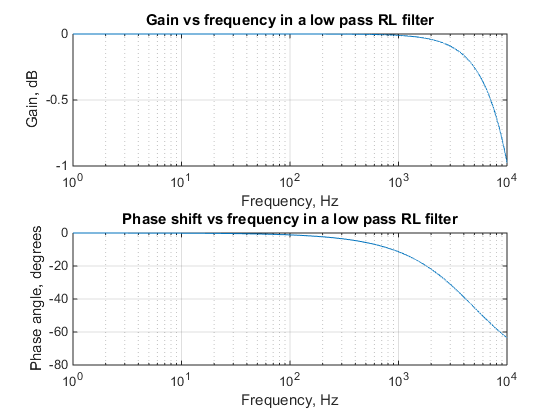
\includegraphics[scale=0.8]{bode2}
			\captionof{figure}{Theoretical bode plots for low pass RL filter}
		\end{minipage}
	\end{figure}
\end{center}

\item[Cut-off frequency for RL low pass filter]
The definition of cut-off frequency that has been widely used by electrical engineers is the frequency for which the transfer function magnitude is decreased by the factor of $\frac{1}{\sqrt{2}}$ from its maximum value. That is:

\begin{align*}
|H(\omega_c)| = \frac{1}{\sqrt{2}}H_{max}
\end{align*}

For a low pass RL circuit, the magnitude of the transfer function is at its maximum when $\omega = 0$, that is $H_{max} = 1$. Hence, setting $|H(\omega_c)|$ equal to $\frac{1}{\sqrt{2}}$ we get:

\begin{align*}
\frac{R}{\sqrt{R^2 + (\omega_c L)^2}} &= \frac{1}{\sqrt{2}} \\
\frac{R^2}{R^2 + (\omega_c L)^2} &= \frac{1}{2} \\
2R^2 &= R^2 + (\omega_c L)^2 \\
R^2 &= (\omega_c L)^2 \\
R &= \omega_c L
\end{align*}

Hence, for a low pass RL circuit, the cut off frequency is given by:

\begin{align}
\omega_c &= \frac{R}{L}
\end{align}

Now, suppose the RL circuit was constructed using a 75 $\si{\ohm}$ resistor and a 2.4 $\si{\milli \henry}$ inductor. The cut off frequency in radians per second would be:

\begin{align*}
	\omega_c &= \frac{75}{2.4e^{-3}} \\
	&= 31250 \si{\sfrac{\radian}{\second}}
\end{align*}

Hence, the cutoff frequency in Hertz is:

\begin{align*}
	f_c = 4973.59 \si{\hertz}
\end{align*}

\end{description} 

\newpage

%----------------------------------------------------------------------------------------
%	SECTION 2
%----------------------------------------------------------------------------------------

\section{Experimental Circuit Set-up, Results and Calculations}

The simple series RC circuit was set up as shown in figure 4. The input voltage, $V_{in}$, was a sinusoidal voltage source generated by the function generator. The output voltage, $V_{out}$, was measured across the capacitor.

%Circuit Diagram
\begin{figure}[H]
\centering
\ctikzset {bipoles/length=.8cm}
\begin{circuitikz}[scale=0.6]
		
		\draw (0,0)
		to [sV, l=$V_{in}$] (0,4)
		to [R, l=330\si{\ohm}] (4,4)
		to [C, v^<=0.47\si{\micro\farad}] (4,0)
		to [short] (0,0)
		;
		
\end{circuitikz}
\captionof{figure}{Series RC circuit with Sinusoidal Input Voltage}
\label{fig:figure2}
\end{figure}

The input voltage, $V_{in}$, was set to 4V peak to peak. Both the output voltage, $V_{out}$, and the time difference between the input signal peak and output signal peak, $|\Delta X|$, were measured. The gain and phase shift were calculated using the formulas from practical 1. The empirical data and calculated values can be seen in table 1.
 
\begin{figure}[H]
\centering
\begin{tabular}{ | r | r | r | r | r | r | }
	\hline
	frequency ($f$) & $V_{in}$ & $V_{out}$ & $|\Delta X|$ & Gain $\si{\decibel}$ & Phase Shift $\si{\degree}$ \\ \hline
	10 \si{\hertz} & 4 \si{\volt} & 4 \si{\volt} & 0 \si{\micro\second} & 0 \si{\decibel} & 0 \si{\degree}\\ \hline
	20 \si{\hertz} & 4 \si{\volt} & 4 \si{\volt} & 0 \si{\micro\second} & 0 \si{\decibel} & 0 \si{\degree}\\ \hline
	50 \si{\hertz} & 4 \si{\volt} & 4 \si{\volt} & 0 \si{\micro\second} & 0 \si{\decibel} & 0 \si{\degree}\\ \hline
	100 \si{\hertz} & 4 \si{\volt} & 4 \si{\volt} & 0 \si{\micro\second} & 0 \si{\decibel} & 0 \si{\degree}\\ \hline
	200 \si{\hertz} & 4 \si{\volt} & 4 \si{\volt} & 200 \si{\micro\second} & 0 \si{\decibel} & -14.4 \si{\degree}\\ \hline
	500 \si{\hertz} & 4 \si{\volt} & 3.6 \si{\volt} & 184 \si{\micro\second} & -0.915 \si{\decibel} & -33.12 \si{\degree}\\ \hline
	1000 \si{\hertz} & 4 \si{\volt} & 2.88 \si{\volt} & 132 \si{\micro\second} & -2.853 \si{\decibel} & -47.52 \si{\degree}\\ \hline
	2000 \si{\hertz} & 4 \si{\volt} & 1.92 \si{\volt} & 90 \si{\micro\second} & -6.375 \si{\decibel} & -64.80 \si{\degree}\\ \hline
	4000 \si{\hertz} & 4 \si{\volt} & 1.12 \si{\volt} & 52 \si{\micro\second} & -11.057 \si{\decibel} & -74.88 \si{\degree}\\ \hline
	5000 \si{\hertz} & 4 \si{\volt} & 1 \si{\volt} & 44 \si{\micro\second} & -12.041 \si{\decibel} & -79.20 \si{\degree}\\ \hline
	8000 \si{\hertz} & 4 \si{\volt} & 0.6 \si{\volt} & 28 \si{\micro\second} & -16.478 \si{\decibel} & -80.64 \si{\degree}\\ \hline
	10000 \si{\hertz} & 4 \si{\volt} & 0.456 \si{\volt} & 24 \si{\micro\second} & -18.861 \si{\decibel} & -86.40 \si{\degree}\\ \hline
\end{tabular}
\captionof{table}{Output characteristics for low pass RC circuit}
\end{figure}

By adjusting the frequency of the function generator until the output voltage had an amplitude of 2.828 $\si{V_{pp}}$, the cut off frequency was measured. The measured value was:

\begin{align*}
	f_c = 995 \si{\hertz}
\end{align*}

\newpage
%%%%%%%%%%%%%%%%%%%%%%%%%%%%%%%%%%%%%%%%%%%%%%%%%%%%%%%%%%%%%%%%%%%%%%%%%%%%%%%%%%%%%%%%%%%

A simple RL circuit was set up as shown in figure 5. The input voltage, $V_{in}$, was a sinusoidal voltage source generated by the function generator. The output voltage, $V_{out}$, was measured across the resistor.

%Circuit Diagram
\begin{figure}[H]
	\centering
	\ctikzset {bipoles/length=.8cm}
	\begin{circuitikz}[scale=0.6]
		
		\draw (0,0)
		to [sV, l=$V_{in}$] (0,4)
		to [L, l=2.4\si{\milli\henry}] (4,4)
		to [R, v^<=75\si{\ohm}] (4,0)
		to [short] (0,0)
		;
		
	\end{circuitikz}
	\captionof{figure}{Series RL circuit with Sinusoidal Input Voltage}
	\label{fig:figure2}
\end{figure}

The input voltage, $V_{in}$, was set to 4V peak to peak. Both the output voltage, $V_{out}$, and the time difference between the input signal peak and output signal peak, $|\Delta X|$, were measured. The gain and phase shift were calculated using the formulas from practical 1. The empirical data and calculated values can be seen in table 2.

\begin{figure}[H]
	\centering
	\begin{tabular}{ | r | r | r | r | r | r | }
		\hline
		frequency ($f$) & $V_{in}$ & $V_{out}$ & $|\Delta X|$ & Gain $\si{\decibel}$ & Phase Shift $\si{\degree}$ \\ \hline
		10 \si{\hertz} & 4 \si{\volt} & 4 \si{\volt} & 0 \si{\micro\second} & 0 \si{\decibel} & 0 \si{\degree}\\ \hline
		20 \si{\hertz} & 4 \si{\volt} & 4 \si{\volt} & 0 \si{\micro\second} & 0 \si{\decibel} & 0 \si{\degree}\\ \hline
		50 \si{\hertz} & 4 \si{\volt} & 4 \si{\volt} & 0 \si{\micro\second} & 0 \si{\decibel} & 0 \si{\degree}\\ \hline
		100 \si{\hertz} & 4 \si{\volt} & 4 \si{\volt} & 0 \si{\micro\second} & 0 \si{\decibel} & 0 \si{\degree}\\ \hline
		200 \si{\hertz} & 4 \si{\volt} & 4 \si{\volt} & 0 \si{\micro\second} & 0 \si{\decibel} & 0 \si{\degree}\\ \hline
		500 \si{\hertz} & 4 \si{\volt} & 4 \si{\volt} & 0 \si{\micro\second} & 0 \si{\decibel} & 0 \si{\degree}\\ \hline
		1000 \si{\hertz} & 4 \si{\volt} & 3.88 \si{\volt} & 48 \si{\micro\second} & -0.265 \si{\decibel} & -17.28 \si{\degree}\\ \hline
		2000 \si{\hertz} & 4 \si{\volt} & 3.60 \si{\volt} & 38 \si{\micro\second} & -0.915 \si{\decibel} & -27.36 \si{\degree}\\ \hline
		4000 \si{\hertz} & 4 \si{\volt} & 2.96 \si{\volt} & 32 \si{\micro\second} & -2.615 \si{\decibel} & -46.08 \si{\degree}\\ \hline
		5000 \si{\hertz} & 4 \si{\volt} & 2.72 \si{\volt} & 28.8 \si{\micro\second} & -3.349 \si{\decibel} & -51.84 \si{\degree}\\ \hline
		8000 \si{\hertz} & 4 \si{\volt} & 2.04 \si{\volt} & 22 \si{\micro\second} & -5.848 \si{\decibel} & -63.36 \si{\degree}\\ \hline
		10000 \si{\hertz} & 4 \si{\volt} & 1.54 \si{\volt} & 18 \si{\micro\second} & -8.291 \si{\decibel} & -64.8 \si{\degree}\\ \hline
	\end{tabular}
	\captionof{table}{Output characteristics for low pass RL circuit}
\end{figure}

By adjusting the frequency of the function generator until the output voltage had an amplitude of 2.828 $\si{V_{pp}}$, the cut off frequency was measured. The measured value was:

\begin{align*}
f_c = 4500 \si{\hertz}
\end{align*}

\newpage


%----------------------------------------------------------------------------------------
%	SECTION 3
%----------------------------------------------------------------------------------------

\section{Results and Conclusions}

The gain and phase angle calculations made for the empirical data shown in tables 1 and 2 for both the RC and RL circuits, respectively, were plotted over the theoretical plots. This can be seen in figure 7 for the RC circuit and figure 8 for the RL circuit.

\begin{center}
	\begin{figure}[H]
		\begin{minipage}{0.6\textwidth}
			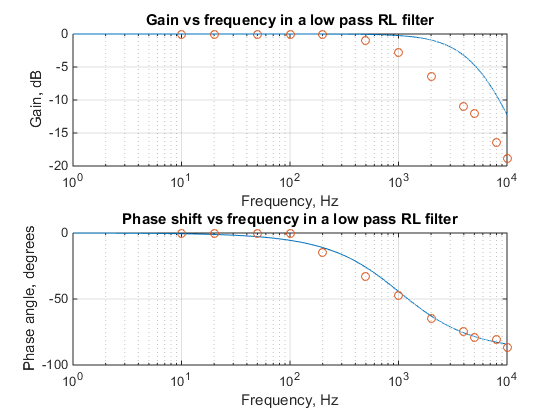
\includegraphics[scale=0.8]{bode3}
			\captionof{figure}{Empirical data super-imposed on theoretical data for low pass RC filter}
		\end{minipage}
	\end{figure}
\end{center}

\begin{center}
	\begin{figure}[H]
		\begin{minipage}{0.6\textwidth}
			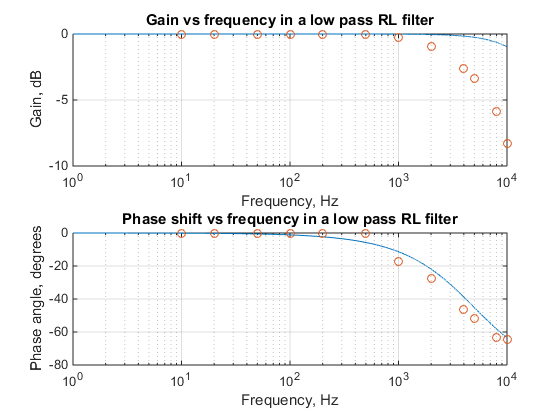
\includegraphics[scale=0.8]{bode4}
			\captionof{figure}{Empirical data super-imposed on theoretical data for low pass RL filter}
		\end{minipage}
	\end{figure}
\end{center}

From figures 7 and 8 we can see that the empirical phase angle data fits the theoretical data well, however, the empirical data for both magnitude plots is attenuated earlier than the theory predicts. This is true for both plots. This early attenuation can also be observed in the difference in the theoretical cut off frequencies and the measured cut off frequencies - both measured cut off frequencies are lower than the theoretical ones. One explanation for the differences in the observed and theoretical values is that the theory assumes that wires in the circuits are perfect conductors and that basic circuit elements operate perfectly. In practice this is simply not true. Wires conducting circuits are not perfect conductors, rather, they carry some resistance. It is this resistance which could impact on the gain of the circuit. Moreover, in most circuits there are parasitic inductive and capacitive effects which would further contribute to the differences in theoretical and observed results.

%----------------------------------------------------------------------------------------
%	BIBLIOGRAPHY
%----------------------------------------------------------------------------------------


%----------------------------------------------------------------------------------------


\end{document}